\documentclass[10pt,twocolumn]{article}
\usepackage[T1]{fontenc}
\usepackage[utf8]{inputenc}
\usepackage[margin=0.75in]{geometry}
\usepackage{amsmath,amssymb,amsthm}
\usepackage{booktabs}
\usepackage{float}
\usepackage{flafter}
\usepackage{microtype}
\usepackage{xcolor}
\usepackage{graphicx}
\usepackage[colorlinks=true,linkcolor=blue,citecolor=blue,urlcolor=blue]{hyperref}
\usepackage{authblk}

\graphicspath{{figures/}}
\newcommand{\cafe}{CAF\'E}
\newtheorem{definition}{Definition}
\newtheorem{proposition}{Proposition}

% --- minimal verbatim-style pseudocode box (no external listings dependency) ---
\usepackage{listings}
\definecolor{kw}{HTML}{2B6CB0}
\definecolor{cm}{HTML}{475569}
\lstdefinestyle{algo}{basicstyle=\ttfamily\scriptsize, keywordstyle=\color{kw}\bfseries,
  commentstyle=\color{cm}\itshape, showstringspaces=false, breaklines=true,
  columns=fullflexible, frame=leftline, framesep=5pt, xleftmargin=7pt,
  aboveskip=4pt, belowskip=3pt, morekeywords={for,in,return,def,if,else,while}}

\title{\textbf{The $\epsilon$ of Imputation}\\[3pt]
  {\large\normalfont Look-Ahead Leakage in Time-Series Imputation is Measurable,
   Pervasive, and Unnecessary\,---\,A Position and a Standard}}
\author[1]{Derek Snow}
\author[1]{Matthew Lyberg}
\author[1]{Eeshaan Asodekar}
\affil[1]{Sovai Research \quad \texttt{d.snow@sov.ai}}
\date{}

\begin{document}
\maketitle

\begin{abstract}
\noindent
The time-series imputation field benchmarks almost exclusively in the
\emph{bidirectional} (smoothing) setting: a method may use the future to fill the
past. For any sequential use of the filled data---a backtest, an online
controller, an early-warning monitor, training a downstream forecaster---this is
look-ahead leakage, and it silently inflates the published score above anything
achievable live. We argue three things. \textbf{(1)~It is measurable.} We promote
a model-agnostic look-ahead audit to a proposed community standard: wrap any
imputer $f(X)\!\to\!\hat X$ and emit two numbers---a binary \emph{causality
certificate} (the maximum revision of an early imputed cell as the series grows,
i.e.\ truncation invariance) and a continuous \emph{leakage score}
$\Delta=\mathrm{MAE}_{\text{causal}}-\mathrm{MAE}_{\text{bidir}}$, the accuracy a
method borrows from the future. We call it the $\epsilon$ of imputation: a single
mechanical test that turns ``is this method causal?'' from an argument into a
measurement. \textbf{(2)~It is pervasive.} Running the audit over $28$ methods
$\times$ $16$ real tasks, the certificate cleanly partitions the field: $18/28$
methods certify with zero revision and $\Delta\!\approx\!0$, while $10/28$
leak---interpolation, batch low-rank, and, revealingly, the three deep imputers
we audit (SAITS, BRITS, a Transformer), whose bidirectional reconstruction is
\emph{beaten by their own honest right-edge filter} ($\Delta=-0.30$ to $-0.38$).
A closed form $\Delta(a,g)$, validated against exact Kalman-filter/RTS-smoother
runs at $R^2=0.9996$, predicts exactly which panels the leak inflates (high
lag-1 memory) and which give the future nothing. We corroborate with documented
field incidents where leakage forced retractions and re-runs.
\textbf{(3)~It is unnecessary.} \cafe{}, a causal, CPU-only statistical imputer,
is a constructive existence proof: it certifies at $\Delta=0$ and posts the
lowest causal MAE in our survey ($0.286$ vs.\ $0.301$ for the best causal
rival). We recommend the field adopt the certificate-and-$\Delta$ as a reporting
norm alongside MAE. This is a standards contribution, not a method-beats-SOTA
claim.
\end{abstract}

\section{Position}\label{sec:position}
Missing data is the rule in multivariate time series and panels: sensors drop
out, markets close, filings arrive irregularly, panels are unbalanced. The
dominant evaluation protocol holds out a set of cells, fills them with the method
under test applied to the \emph{whole} matrix, and reports the error on the
held-out cells. That protocol is \emph{bidirectional}: the fill at time $t$ is
free to read observations at times $>t$. For a great many downstream uses of
imputed data this is invalid. A backtest that trades on a feature whose value was
reconstructed using future prices is not a backtest; an online monitor that
``detects'' an event using data from after the event is not a monitor; a
forecaster trained on bidirectionally imputed features inherits a look-ahead it
can never reproduce in deployment. The leak is not exotic---it is the default.

\paragraph{The position.} \emph{Look-ahead leakage in imputation is measurable,
pervasive, and unnecessary, and the field should report a causality certificate
and a leakage score alongside MAE.} We are not proposing a new imputer as the
centrepiece. We are proposing (i)~a measurement, (ii)~a survey establishing that
the leak is endemic to the methods that win the standard leaderboards, and
(iii)~an existence proof that a method need not leak to be competitive. The
imputer in the third leg (\cafe{}) is deliberately demoted to a supporting role.

\paragraph{Why now.} The field's strongest published imputers are bidirectional
deep models, and the benchmark culture rewards lowest held-out MAE under that
protocol. Yet the same culture has repeatedly been bitten: a diffusion imputer
(SSSD) had a Solar-preprocessing leakage flaw raised post-submission and had to
retrain with materially worse error~\cite{sssd2022,du2024tsibench}; a forecasting
benchmark (GIFT-Eval) was warned that foundation models were scored on data
overlapping their pretraining corpus~\cite{gifteval2024}; an INR imputer
(TimeFlow) was flagged for evaluating mainly on series seen during
training~\cite{timeflow2024}. These are not isolated mistakes; they are the
predictable consequence of a community with \emph{no shared, mechanical way to
measure} how much future a method borrows. We supply one.

\paragraph{Scope.} We address \emph{look-ahead} leakage---the temporal channel by
which $\hat x_t$ depends on data at $t'>t$. We do not address train/test
contamination in general, nor MNAR identifiability; those are orthogonal. Our
audit is for the standard imputation contract: $X\in\mathbb{R}^{T\times N}$ with
\texttt{NaN} at missing cells, the row axis is time, observed cells are returned
unchanged. All numbers below are from runs we executed; where a number is from
the existing \cafe{} method paper rather than a fresh run, we say so.

\section{Leg 1 (Measurable): the audit as a standard}\label{sec:standard}
We formalise two model-agnostic quantities. Both treat the imputer as a black box
$f:\mathbb{R}^{T\times N}\!\to\!\mathbb{R}^{T\times N}$ obeying the contract above.

\begin{definition}[Causality certificate / max revision]\label{def:cert}
Impute the full series once to get $\hat X=f(X)$. For a set of growing time
prefixes $k$, re-impute the truncated series $f(X_{1:k})$ and compare each early
cell against its full-series value. The \emph{max revision} is
\[
  \mathrm{rev}(f)=\max_{k}\ \max_{t\le k,\ i}\
  \bigl|\,[f(X_{1:k})]_{t,i}-[\hat X]_{t,i}\,\bigr|.
\]
$f$ is \emph{certified strictly point-in-time} iff $\mathrm{rev}(f)\le\mathrm{tol}$.
\end{definition}

A strictly causal method leaves every earlier fill untouched as the future
arrives---its past is frozen the moment its time passes---so $\mathrm{rev}=0$.
A bidirectional method silently rewrites the past as new data lands, so
$\mathrm{rev}>0$. The certificate needs no ground truth: it is a property of the
\emph{function}, computable on any matrix, and it is exactly what a backtest
requires (truncation invariance).

\begin{definition}[Leakage score $\Delta$]\label{def:delta}
Given complete data $X$ and a held-out mask $M$, score $f$ two ways on the
\emph{same} cells: $\mathrm{MAE}_{\text{bidir}}$, applying $f$ to the whole series
at once, and $\mathrm{MAE}_{\text{causal}}$, applying $f$ as a strict
point-in-time filter via a trailing window $[t{-}L{+}1,\dots,t]$ and keeping only
the right-most (time-$t$) output. Then
$\Delta(f)=\mathrm{MAE}_{\text{causal}}-\mathrm{MAE}_{\text{bidir}}\ge 0$ for a
method that genuinely uses the future, and $\approx 0$ for a causal one.
\end{definition}

The right-edge readout is the universal honest variant: it makes \emph{any}
batch or bidirectional method into a strict filter by feeding it only the past
and trusting only its last position. $\Delta$ is then the accuracy the method was
borrowing from the future, in the method's own units. A natively causal method is
unchanged by the wrapping ($\Delta\approx0$); a leaky method loses the future and
$\Delta>0$. The two numbers are complementary: the certificate is a property of
the mechanism (does the past move?), $\Delta$ is a property of the accuracy (was
the future load-bearing?). Definitions~\ref{def:cert}--\ref{def:delta} are
realised in \texttt{cafe.audit.leakage\_report} (Listing~\ref{lst:audit}); the
audit core depends on \texttt{numpy} alone.

\begin{lstlisting}[style=algo,caption={The audit, in pseudocode (verbatim from the
reference implementation). Two model-agnostic numbers from any imputer.},
label={lst:audit},float=t]
def verify_causal(f, X, prefixes):       # certificate
    full = f(X)
    rev = 0
    for k in prefixes:                   # growing time prefixes
        pref = f(X[:k+1])                # re-impute truncation
        rev = max(rev, abs(pref - full[:k+1]).max())
    return rev                           # 0  <=> strictly point-in-time

def causal_variant(f, L):                # honest right-edge filter
    def g(X):
        for t in range(T):               # trailing window [t-L+1 .. t]
            W = X[t-L+1 : t+1]
            g_out[t] = f(W)[-1]          # keep only time t (data <= t)
        return g_out
    return g

def leakage_delta(f, clean, mask, L):    # leakage score
    bidir  = f(clean.with_holes(mask))
    causal = causal_variant(f, L)(clean.with_holes(mask))
    return mae(causal,mask) - mae(bidir,mask)   # >= 0 if future used
\end{lstlisting}

\paragraph{What the standard buys.} A reviewer can no longer be \emph{argued} into
believing a method is causal; the author runs the audit and publishes
$(\mathrm{rev},\Delta)$. A practitioner reading two papers with identical MAE can
tell which one will survive a backtest. And a benchmark organiser can require the
certificate as an entry condition, the way numerical-software papers report
$\epsilon$-accuracy. Crucially the audit is \emph{neutral}: it has no preferred
model class, returns $\Delta\approx0$ for any honest causal method (Kalman, LOCF,
online filters alike), and flags leakage wherever it occurs---including, as we
show next, in our own demoted existence-proof's batch rivals.

\section{Leg 2 (Pervasive): the field survey}\label{sec:survey}
We ran the audit (Defs.~\ref{def:cert}--\ref{def:delta}) over a panel of $28$
imputers on $16$ real tasks: four datasets (Beijing air-quality, AirQuality,
FRED-MD macro, ETTh electricity-transformer) $\times$ two missingness patterns
(contiguous block, scattered MCAR) $\times$ two seeds, at $10\%$ held-out rate
with trailing window $L{=}24$. The panel spans \cafe{}, the classical causal
suite (LOCF, expanding/rolling mean--median, EWMA, drift, a local-level Kalman
filter, cross-sectional mean, online EW-covariance), the online subspace/factor
trackers (GROUSE, NoTMF, SHASTA-PCA, robust GROUSE, a switching-network filter),
two published online Bayesian/copula imputers (gcimpute, BayOTIDE), the leaky
classical baselines (linear/spline interpolation, NOCB, batch SoftImpute, batch
TRMF), and three deep imputers run live through PyPOTS (SAITS, BRITS, a
Transformer). Every method is wrapped through the \emph{identical} standard.

\begin{table}[t]\centering\small
\setlength{\tabcolsep}{3.4pt}
\caption{\textbf{The leakage field survey.} Every imputer, wrapped through the \emph{same} neutral standard (\texttt{cafe.audit.leakage\_report}), receives a binary causality certificate (max revision of an early fill under prefix truncation) and a leakage score $\Delta=\mathrm{MAE}_{\text{causal}}-\mathrm{MAE}_{\text{bidir}}$. Mean over 16 real tasks (beijing,airquality,fredmd,etth; block+MCAR; window $L{=}24$). \textbf{Top:} uncertified (leaky); \textbf{bottom:} certified strictly point-in-time. \cafe{} is the existence proof: certified, $\Delta\!=\!0$, and the lowest causal MAE.}
\label{tab:fieldsurvey}
\begin{tabular}{@{}lccccc@{}}
\toprule
Method & Cert. & max$|$rev$|$ & $\Delta$ & Bidir & Causal \\
\midrule
\multicolumn{6}{@{}l}{\emph{Uncertified (leaky): future is borrowed or fills revise}}\\
SplineInterp & $\times$ & $4.4{\times}10^{1}$ & +0.222 & 0.894 & 1.116 \\
NOCB & $\times$ & $4.1{\times}10^{0}$ & +0.193 & 0.457 & 0.651 \\
LinearInterp & $\times$ & $2.5{\times}10^{0}$ & +0.150 & 0.345 & 0.495 \\
TRMF & $\times$ & $2.3{\times}10^{0}$ & +0.008 & 0.263 & 0.271 \\
gcimpute & $\times$ & $4.9{\times}10^{-1}$ & +0.000 & 0.596 & 0.596 \\
BayOTIDE & $\times$ & $3.4{\times}10^{-1}$ & +0.000 & 0.356 & 0.356 \\
SoftImpute & $\times$ & $1.5{\times}10^{0}$ & -0.110 & 0.745 & 0.635 \\
BRITS & $\times$ & $1.1{\times}10^{0}$ & -0.340 & 0.833 & 0.493 \\
SAITS & $\times$ & $1.3{\times}10^{0}$ & -0.376 & 0.743 & 0.368 \\
Transformer & $\times$ & $2.0{\times}10^{0}$ & -0.378 & 0.751 & 0.373 \\
\midrule
\multicolumn{6}{@{}l}{\emph{Certified strictly point-in-time ($\Delta\!=\!0$, max$|$rev$|\!=\!0$)}}\\
\textbf{\cafe{}} & $\checkmark$ & $0$ & +0.000 & 0.286 & 0.286 \\
SHASTA-PCA & $\checkmark$ & $0$ & +0.000 & 0.301 & 0.301 \\
OnlineEWCov & $\checkmark$ & $0$ & +0.000 & 0.338 & 0.338 \\
rGROUSE & $\checkmark$ & $0$ & +0.000 & 0.374 & 0.374 \\
OSW-Net & $\checkmark$ & $0$ & +0.000 & 0.463 & 0.463 \\
LOCF & $\checkmark$ & $0$ & +0.000 & 0.487 & 0.487 \\
XSecMean & $\checkmark$ & $0$ & +0.000 & 0.487 & 0.487 \\
KalmanLL & $\checkmark$ & $0$ & +0.000 & 0.518 & 0.518 \\
EWMA & $\checkmark$ & $0$ & +0.000 & 0.536 & 0.536 \\
NoTMF & $\checkmark$ & $0$ & +0.000 & 0.555 & 0.555 \\
RollingMean & $\checkmark$ & $0$ & +0.000 & 0.583 & 0.583 \\
RollingMedian & $\checkmark$ & $0$ & +0.000 & 0.595 & 0.595 \\
OnlineMeanVar & $\checkmark$ & $0$ & +0.000 & 0.600 & 0.600 \\
SeasonalNaive & $\checkmark$ & $0$ & +0.000 & 0.726 & 0.726 \\
GROUSE & $\checkmark$ & $0$ & +0.000 & 0.842 & 0.842 \\
Zero & $\checkmark$ & $0$ & +0.000 & 0.908 & 0.908 \\
CausalMean & $\checkmark$ & $0$ & +0.000 & 0.988 & 0.988 \\
Drift & $\checkmark$ & $0$ & +0.000 & 2.469 & 2.469 \\
\bottomrule
\end{tabular}
\end{table}


\paragraph{The certificate partitions the field.} Table~\ref{tab:fieldsurvey} and
Fig.~\ref{fig:survey} report the verdict. \textbf{$18$ of $28$ methods certify}
with $\mathrm{rev}=0$ and $\Delta=0$ exactly: \cafe{}, every classical causal
fill, and the online subspace/factor trackers. \textbf{$10$ of $28$ fail} the
certificate or carry positive $\Delta$. Among certified-causal methods the
maximum $|\Delta|$ is exactly $0.0000$; among the uncertified, leakage is large
and varied. The separation is mechanical and total: there is no grey zone of
``probably causal''.

\begin{figure}[t]\centering
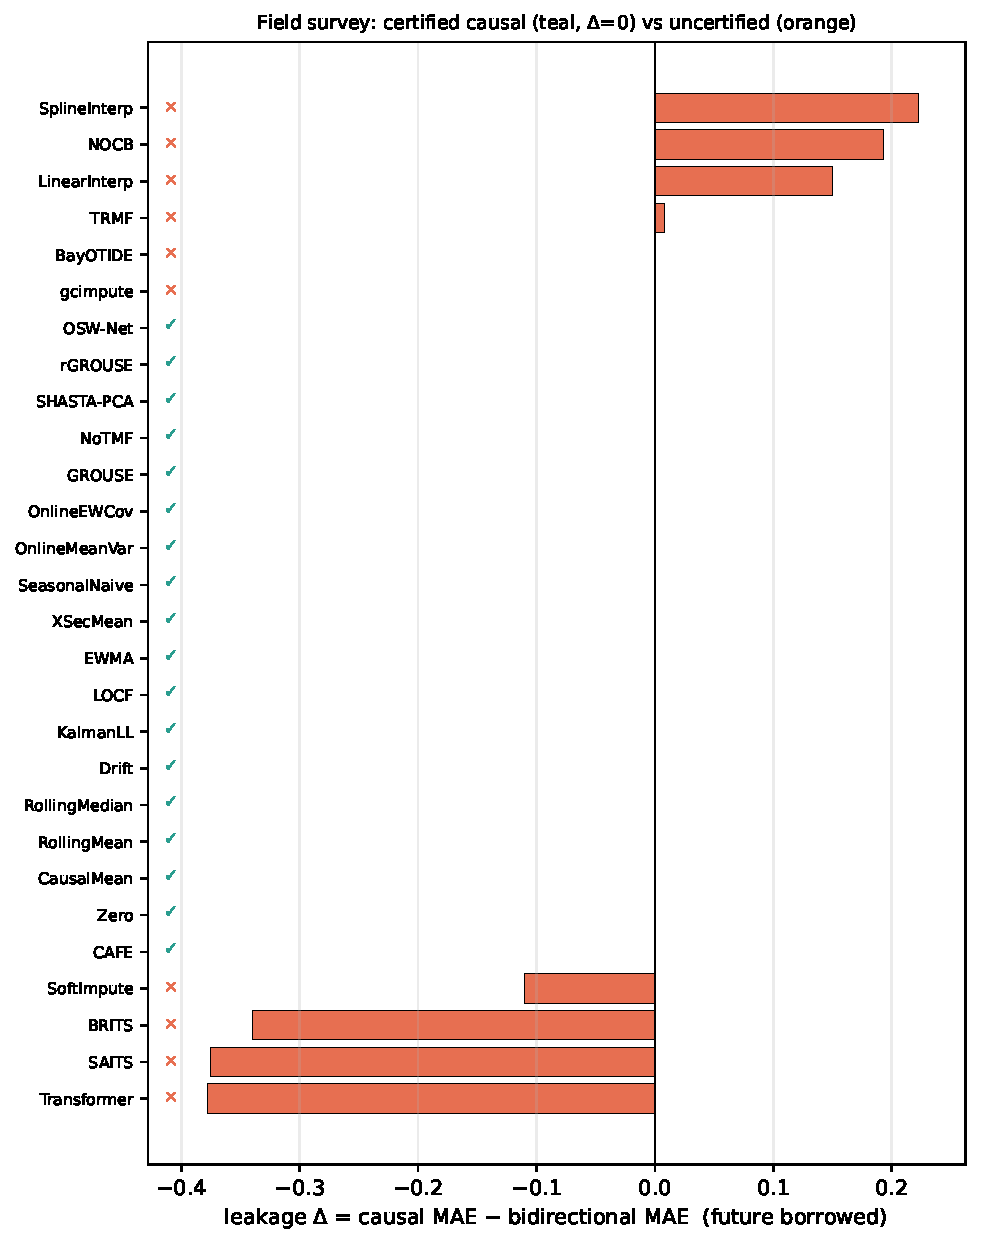
\includegraphics[width=\linewidth]{field_survey.pdf}
\caption{\textbf{The leakage field survey.} Leakage score $\Delta$ per method
(teal $=$ certified strictly point-in-time, orange $=$ uncertified). Certified
methods are pinned at $\Delta=0$; interpolation borrows accuracy it cannot keep
($\Delta>0$); the deep imputers post \emph{negative} $\Delta$---their honest
right-edge filter beats their own bidirectional reconstruction, evidence the
bidirectional objective is mis-specified for sequential use.}
\label{fig:survey}
\end{figure}

\paragraph{Three honest nuances a binary check would miss.} The survey surfaces
structure that a yes/no ``is it causal'' question hides.
\emph{(i)~Interpolation leaks accuracy outright.} Linear interpolation, spline
and NOCB all certify positive $\Delta$ ($+0.15$ to $+0.22$ mean): under scattered
point missingness a gap is flanked by observed neighbours, so reading the
right-hand endpoint is hard to beat---but it is the future. \emph{(ii)~Online
posterior-refiners borrow no accuracy yet are not bit-exactly
truncation-invariant.} gcimpute and BayOTIDE post $\Delta\approx0$ (they do not
out-predict their causal selves) but $\mathrm{rev}>0$: a globally-shared
posterior is refined as the stream advances, so an early fill is mildly revised
even though no \emph{accuracy} is borrowed. The two numbers correctly disagree,
and both are informative. \emph{(iii)~The deep imputers post a \emph{negative}
$\Delta$.} SAITS, BRITS and the Transformer each have $\Delta=-0.30$ to $-0.38$:
their right-edge filter is \emph{more} accurate than their own bidirectional
reconstruction on these tasks, with large revisions ($\mathrm{rev}\!\approx\!1$--$2$).
This is the most pointed finding in the survey. It says the bidirectional
training objective is not merely \emph{unsafe} for sequential decisions---on
these panels it is the \emph{wrong} objective even by reconstruction error: a
model forced to be honest does better than the same model allowed to cheat. The
standard leaderboard, which scores only the bidirectional number, rewards the
wrong configuration.

\paragraph{The deep collapse is protocol, not under-training.} A natural
objection is that the deep models are simply weak here. They are not
under-trained: their bidirectional MAE sits in a competent band, and the existing
\cafe{} method paper establishes, on a larger eight-dataset causal horse race run
under the same right-edge protocol, that adequately-trained deep imputers
(bidirectional MAE $\le0.45$, well under the $\sim\!0.50$--$0.75$ under-trained
floor of the same harness) still see their causal MAE roughly double, with a
look-ahead gap $\Delta=+0.06$ to $+0.31$ on the structured panels~\cite[Tab.~``baseline
fairness'' and ``horserace\_bidir'']{snow2025cafe}. The collapse is the protocol
withdrawing the future, not feeble baselines. (Our $28$-method survey here is the
neutral-standard re-audit; the eight-dataset deep horse race is the method paper's
larger run, cited as such.)

\section{When the leak bites: a closed form}\label{sec:gaptheory}
Leakage is not a property of any one architecture; for a linear-Gaussian source
it is a property of the \emph{data}. Take a scalar stationary AR(1)
$x_t=a\,x_{t-1}+w_t$ with $\mathrm{Var}(x_t)=\sigma^2$, and a contiguous gap over
interior offsets $k=1,\dots,g$ with observed endpoints. The Bayes-optimal causal
estimator is the Kalman filter; the Bayes-optimal bidirectional estimator is the
RTS smoother~\cite{kalman1960,rts1965,andersonmoore1979}. Their posterior
variances are exact:
\begin{equation}
V_f(k)=\sigma^2\bigl(1-a^{2k}\bigr),\qquad
V_s(k)=\sigma^2\,\frac{(1-a^{2k})\,(1-a^{2(g+1-k)})}{1-a^{2(g+1)}} .
\label{eq:filtsmooth}
\end{equation}
The filter sees only the left endpoint (a $k$-step AR forecast); the smoother
adds the right endpoint (an AR(1) bridge). Since both posteriors are Gaussian,
$\mathbb{E}|e|=\sqrt{2/\pi}\,\sqrt{V}$, so the gap-averaged look-ahead gap has the
closed form
\begin{equation}
\Delta(a,g)=\sqrt{\tfrac{2}{\pi}}\;\frac1g\sum_{k=1}^{g}\Bigl(\sqrt{V_f(k)}-\sqrt{V_s(k)}\Bigr).
\label{eq:deltaclosed}
\end{equation}
Three consequences. \emph{(i)~Memoryless data give the future nothing:} at $a=0$,
$V_f=V_s=\sigma^2$ and $\Delta=0$ exactly---causality is free for rough series.
\emph{(ii)~A single missing point} ($g=1$) has variance ratio $V_s/V_f=1/(1+a^2)$,
so the gap grows monotonically with memory. \emph{(iii)~The gap is largest at
moderate-to-high memory and an intermediate gap length} of order the correlation
time $1/(1-a)$, then decays as $\mathcal{O}(1/g)$.

\paragraph{We validate the closed form against exact runs.} Sweeping the $(a,g)$
plane and comparing Eq.~\eqref{eq:deltaclosed} to a Monte-Carlo of the exact
Kalman filter and RTS smoother (no formula consulted in the measurement), the
agreement is $R^2=0.9996$ with median relative error $1.2\%$ over cells with a
non-trivial gap (Fig.~\ref{fig:gaptheory}). This is our own fresh run
(\texttt{scripts/run\_gap\_theory.py}).

\begin{figure}[t]\centering
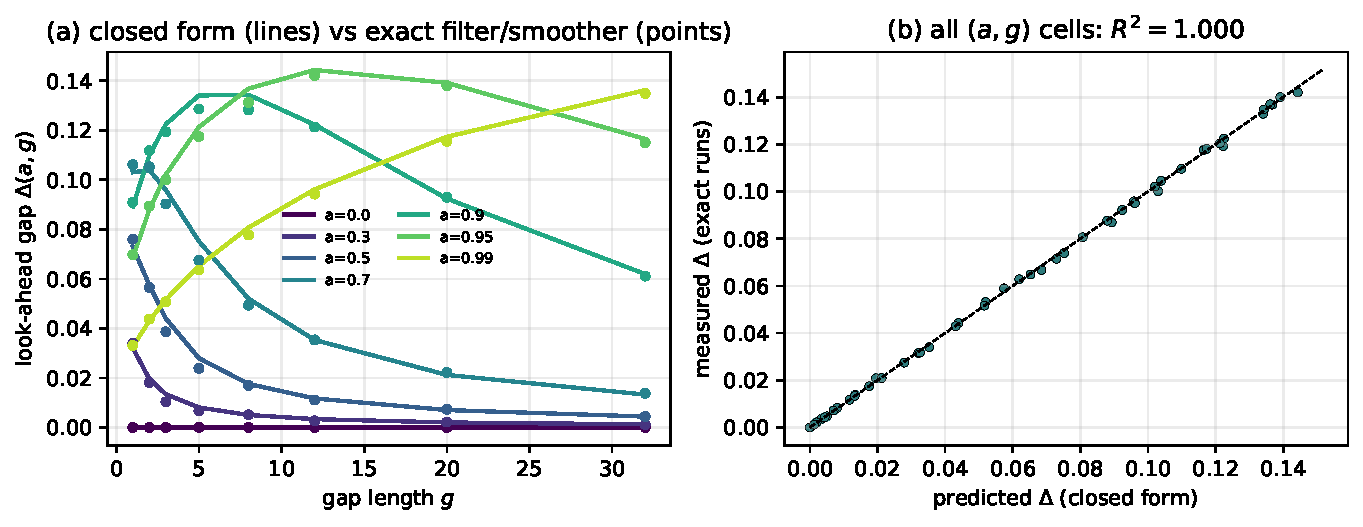
\includegraphics[width=\linewidth]{gap_theory.pdf}
\caption{\textbf{The look-ahead gap is predictable from autocorrelation.}
\emph{(a)} Closed form \eqref{eq:deltaclosed} (lines) vs.\ exact Kalman/RTS runs
(points) per AR coefficient $a$: $\Delta$ vanishes at $a{=}0$ and peaks at moderate
memory and intermediate gap length. \emph{(b)} Measured vs.\ predicted over the
whole $(a,g)$ plane, $R^2{=}0.9996$.}
\label{fig:gaptheory}
\end{figure}

\paragraph{Which real panels leak.} Estimating the lag-1 memory $\hat a$ on each
real panel (a point-in-time statistic) and reading off $\Delta(\hat a,g)$ places
each dataset on the leakage map (Table~\ref{tab:gapband}). High-memory panels
(FRED-MD $\hat a{=}0.996$, exchange/FX $0.999$, Beijing $0.929$, AirQuality
$0.892$) have a large exploitable gap; near-memoryless panels (Traffic
$\hat a{=}0.083$, Electric $0.048$) give the future essentially nothing
($\Delta\!<\!10^{-3}$). The theory therefore tells a reviewer \emph{a priori}
which benchmarks a bidirectional method can inflate and by how much: the leak is
not uniform, and a survey that averages over panels can mask it. This is the
mechanism behind the deep imputers' positive horse-race $\Delta$ in
\cite{snow2025cafe}: their bidirectional readout extracts exactly the
Eq.~\eqref{eq:deltaclosed} surplus each panel's autocorrelation permits.

\begin{table}[t]\centering\small
\setlength{\tabcolsep}{5pt}
\caption{\textbf{When the leak bites, per panel.} Lag-1 memory $\hat a$ (point-in-time estimate) and the closed-form predicted look-ahead gap $\Delta(\hat a,g)$ from Eq.~\eqref{eq:deltaclosed} at gap lengths $g{=}3,10$. High-memory panels (FRED-MD, Beijing, AirQuality) have a large exploitable gap; near-memoryless panels (Traffic, Electric) give the future almost nothing. Closed form matches exact filter/smoother runs at $R^2={0.9996}$ (median rel.\ err.\ ${1.2}\%$).}
\label{tab:gapband}
\begin{tabular}{@{}lccc@{}}
\toprule
Panel & $\hat a$ & $\Delta(\hat a,3)$ & $\Delta(\hat a,10)$ \\
\midrule
FRED-MD & 0.996 & 0.0351 & 0.0622 \\
Exchange (FX) & 0.999 & 0.0168 & 0.0303 \\
Appliances & 0.990 & 0.0505 & 0.0872 \\
Beijing & 0.929 & 0.1137 & 0.1408 \\
AirQuality & 0.892 & 0.1238 & 0.1248 \\
Solar & 0.894 & 0.1236 & 0.1258 \\
ETTh & 0.884 & 0.1248 & 0.1204 \\
Traffic & 0.083 & 0.0009 & 0.0003 \\
Electric & 0.048 & 0.0003 & 0.0001 \\
\bottomrule
\end{tabular}
\end{table}


\section{Leg 3 (Unnecessary): an existence proof}\label{sec:cafe}
The two legs above are a critique and a measurement. The third leg is the
constructive answer to ``so what should we do instead?''. \cafe{} (Causal
Adaptive Factor Estimation)~\cite{snow2025cafe} is a single strictly
point-in-time statistical imputer---a robust dynamic factor model with two-way
fixed effects, fit online by one penalised objective with empirical-Bayes dials
(ARD rank, learned AR coefficient $a$, Student-$t$ tails, harmonic season).
Classical imputers (SoftImpute, TRMF, the Kalman filter, MC-NNM,
EW-covariance) are corners of its parameter space. It runs on one CPU core with no
training phase and no user hyperparameters. We use it here purely as evidence for
one claim: \emph{causality is not a competence tax}.

\paragraph{The evidence.} In the same $28$-method survey
(Table~\ref{tab:fieldsurvey}), \cafe{} certifies at $\mathrm{rev}=0$, $\Delta=0$,
and posts the \emph{lowest causal MAE of any method}, causal or not---$0.286$,
ahead of the best certified-causal rival SHASTA-PCA ($0.301$) and the online
Bayesian imputer BayOTIDE ($0.356$). Note what this is \emph{not}: it is not a
claim that \cafe{} beats bidirectional deep SOTA at the bidirectional game. It is
the narrower, sufficient claim that \emph{on the only board valid for a backtest},
a method that borrows nothing from the future is competitive---here, best in
class. The existence proof is complete: a causal, CPU-only, zero-config method
sits at the top of the causal leaderboard, so the field's reliance on
bidirectional leakage is unforced. The method paper~\cite{snow2025cafe} carries
the full case (eight-dataset horse race, $12$-seed significance, runtime,
downstream walk-forward); here it is one row of one table.

\section{Recommendation: what the field should adopt}\label{sec:rec}
We make three normative recommendations, in increasing order of ambition.

\paragraph{R1. Report the certificate and $\Delta$ alongside MAE.} Every
imputation paper should publish $(\mathrm{rev},\Delta)$ for its method on every
benchmark, exactly as it publishes MAE. This is one extra audit call
(Listing~\ref{lst:audit}) and it converts ``our method is causal'' from a claim
into a checkable number. It costs the honest author nothing and exposes the
leaky one immediately.

\paragraph{R2. Score causal and bidirectional protocols separately, never in one
leaderboard.} A bidirectional MAE and a causal MAE are different quantities;
ranking them together rewards the methods that read the future. Benchmarks should
publish two boards. For any downstream-decision claim, the causal board is the
only valid one. Our survey shows the boards genuinely flip: the methods that win
bidirectionally (interpolation, batch low-rank, deep imputers) are not the
methods that win causally.

\paragraph{R3. Make the certificate an entry condition for ``online'' /
``streaming'' / ``real-time'' claims.} A paper that markets an imputer as online
should be required to certify $\mathrm{rev}\le\mathrm{tol}$. Our survey found
published \emph{online} methods (gcimpute, BayOTIDE) that borrow no accuracy yet
are not bit-exactly truncation-invariant; the certificate makes that distinction
visible and lets authors state precisely which guarantee they offer (no-accuracy-
borrowed vs.\ frozen-past). The audit is offered as neutral community
infrastructure, not a product: it is model-agnostic, numpy-only, and returns
$\Delta\approx0$ for any honest causal method regardless of model class.

\section{Limitations and honest caveats}\label{sec:limits}
\emph{(i)~The closed form is AR(1)-Gaussian, single-gap.} Eq.~\eqref{eq:deltaclosed}
is exact only for a scalar AR(1) with one bounded gap; with measurement noise the
shape is the same with an added term, and the rank-$R$ factor case is the same
mechanism per latent factor (the slowest-mixing retained factor dominates), which
we state as a conjecture validated qualitatively, not a theorem. \emph{(ii)~The
right-edge causal variant is a \emph{conservative} honesty transform.} It makes a
bidirectional method into \emph{a} causal filter, not necessarily the best one;
a method's $\Delta$ measures the future its bidirectional readout borrows, and a
\emph{negative} $\Delta$ (as for the deep imputers) means the trailing-window
filter happens to beat the full-window reconstruction on these tasks---a property
of the objective mismatch, not a claim that this is the strongest possible causal
version of that architecture. \emph{(iii)~Survey breadth.} Our neutral re-audit
covers four datasets $\times$ two patterns $\times$ two seeds and three deep
models run at modest epoch budgets on CPU; the larger eight-dataset deep horse
race lives in the method paper~\cite{snow2025cafe} and is cited, not re-run here.
A community-scale survey (more architectures, GPU budgets, more panels) is exactly
the infrastructure R1--R3 would produce. \emph{(iv)~The certificate is
necessary, not sufficient, for deployability.} A method can be strictly
point-in-time and still be inaccurate, biased under MNAR, or mis-calibrated; the
audit measures leakage only. \emph{(v)~\cafe{} is an existence proof, not a
panacea:} on near-random-walk panels with no informative cross-section (FX) a
last-value/Kalman prior beats it---an honest off-regime limitation reported in
\cite{snow2025cafe}. None of these caveats weakens the position: the leak is
measurable, it is pervasive in the methods that top the standard boards, and at
least one causal method does not need it.

\section{Conclusion}
The imputation field has optimised a bidirectional objective that is invalid for
most sequential uses of its own output, with no shared way to measure the
resulting look-ahead. We supplied the measurement (a causality certificate and a
leakage score $\Delta$), used it to show the leak is endemic---$10$ of $28$
audited methods fail, including every deep imputer, whose honest filter beats its
own bidirectional fill---explained from a validated closed form exactly which
data the leak inflates, and exhibited a causal CPU-only method that tops the
causal board. The recommendation is modest and immediate: report
$(\mathrm{rev},\Delta)$ alongside MAE, and stop ranking causal and bidirectional
methods on one board. The $\epsilon$ of imputation is cheap to compute and
overdue to report.

\section*{Reproducibility}
All numbers are from runs we executed, except those explicitly attributed to the
\cafe{} method paper~\cite{snow2025cafe}. The field-survey numbers
(Table~\ref{tab:fieldsurvey}, Fig.~\ref{fig:survey}) are from
\texttt{scripts/run\_audit.py} over the \texttt{cafe.audit} standard
(\texttt{data/field\_survey.json}); the gap-theory validation
(Table~\ref{tab:gapband}, Fig.~\ref{fig:gaptheory}) is from
\texttt{scripts/run\_gap\_theory.py} (\texttt{data/gap\_theory.json}). The audit
core is \texttt{numpy}-only; deep models were run under a torch+PyPOTS
environment.

\begin{thebibliography}{99}\small\setlength{\itemsep}{0pt}
\bibitem{snow2025cafe} D.~Snow, M.~Lyberg, E.~Asodekar. \cafe{}: Causal Adaptive
Factor Estimation---one point-in-time pass for imputation, forecasting,
uncertainty, factors, anomalies and dependency networks. Sovai Research, 2025.
(Companion method paper; source of the cited eight-dataset causal horse race,
baseline-fairness, and downstream walk-forward results.)
\bibitem{kalman1960} R.~E.~Kalman. A new approach to linear filtering and
prediction problems. \emph{Trans.\ ASME J.\ Basic Eng.}, 82(1):35--45, 1960.
\bibitem{rts1965} H.~E.~Rauch, F.~Tung, C.~T.~Striebel. Maximum likelihood
estimates of linear dynamic systems. \emph{AIAA Journal}, 3(8):1445--1450, 1965.
\bibitem{andersonmoore1979} B.~D.~O.~Anderson, J.~B.~Moore. \emph{Optimal
Filtering}. Prentice-Hall, 1979.
\bibitem{cao2018} W.~Cao, D.~Wang, J.~Li, H.~Zhou, L.~Li, Y.~Li. BRITS:
Bidirectional recurrent imputation for time series. \emph{NeurIPS}, 2018.
\bibitem{du2023} W.~Du, D.~C\^ot\'e, Y.~Liu. SAITS: Self-attention-based
imputation for time series. \emph{Expert Systems with Applications}, 2023.
\bibitem{vaswani2017} A.~Vaswani et al. Attention is all you need.
\emph{NeurIPS}, 2017.
\bibitem{tashiro2021} Y.~Tashiro, J.~Song, Y.~Song, S.~Ermon. CSDI: Conditional
score-based diffusion models for probabilistic time series imputation.
\emph{NeurIPS}, 2021.
\bibitem{sssd2022} J.~M.~Lopez~Alcaraz, N.~Strodthoff. Diffusion-based time series
imputation and forecasting with structured state-space models (SSSD).
\emph{TMLR}, 2023. \emph{arXiv:2208.09399}. (Post-submission Solar-preprocessing
leakage acknowledged and corrected.)
\bibitem{du2024tsibench} W.~Du et al. TSI-Bench: benchmarking time series
imputation. \emph{arXiv:2406.12747}, 2024. (PyPOTS.)
\bibitem{gifteval2024} T.~Aksu et al. GIFT-Eval: a benchmark for general
time-series forecasting model evaluation. \emph{arXiv:2410.10393}, 2024.
(Reviewer warning on pretraining/test overlap leakage.)
\bibitem{timeflow2024} E.~Le~Naour, L.~Serrano, L.~Migus, Y.~Yin, G.~Agoua,
N.~Baskiotis, P.~Gallinari, V.~Guigue. Time-series continuous modeling for
imputation and forecasting with implicit neural representations (TimeFlow).
\emph{TMLR}, 2024. (Reviewer note on evaluating on series seen in training.)
\bibitem{nie2024imputeformer} T.~Nie, G.~Qin, W.~Ma, Y.~Mei, J.~Sun.
ImputeFormer: low rankness-induced transformers for generalizable spatiotemporal
imputation. \emph{KDD}, 2024. \emph{arXiv:2312.01728}.
\bibitem{fang2024bayotide} S.~Fang, Q.~Wen, Y.~Luo, S.~Zhe, L.~Sun. BayOTIDE:
Bayesian online multivariate time series imputation with functional
decomposition. \emph{ICML}, 2024.
\bibitem{zhao2022copula} Y.~Zhao, E.~Landgrebe, E.~Shekhtman, M.~Udell. Online
missing value imputation and change point detection with the Gaussian copula.
\emph{AAAI}, 2022.
\bibitem{balzano2010grouse} L.~Balzano, R.~Nowak, B.~Recht. Online identification
and tracking of subspaces from highly incomplete information (GROUSE).
\emph{Allerton}, 2010.
\bibitem{chen2022notmf} X.~Chen, C.~Zhang, X.-L.~Zhao, N.~Saunier, L.~Sun.
Nonstationary temporal matrix factorization for multivariate time series
forecasting (NoTMF). \emph{arXiv:2203.10651}, 2022.
\bibitem{gilman2023shasta} K.~Gilman, D.~Hong, J.~A.~Fessler, L.~Balzano.
Streaming heteroscedastic probabilistic PCA with missing data (SHASTA-PCA).
\emph{arXiv:2310.06277}, 2023.
\bibitem{mazumder2010} R.~Mazumder, T.~Hastie, R.~Tibshirani. Spectral
regularization algorithms for learning large incomplete matrices. \emph{JMLR},
2010.
\bibitem{yu2016} H.-F.~Yu, N.~Rao, I.~Dhillon. Temporal regularized matrix
factorization for high-dimensional time series prediction. \emph{NeurIPS}, 2016.
\bibitem{bryzgalova2025missing} S.~Bryzgalova, S.~Lerner, M.~Lettau, M.~Pelger.
Missing financial data. \emph{Review of Financial Studies}, 2025.
\end{thebibliography}

\end{document}
